\subsection{Motivation}
Having successfully verified a lane change scenario using the APEX framework we shift our focus to scalability and usability. Scalability in this sense revolves around three key issues: 
\begin{itemize}
	\item As the complexity of scenarios grows (ie the number of agents increase) how can we ensure that verification instances are built quickly and accurately?
	\item As the realism of the controllers used in the scnearios is increased how can we create tractable representations of such systems?
	\item As the language describing the other agents behaviors becomes more expressive can naieve application of verification technology meet the challenge?
\end{itemize}
In order to begin to provide a structured answer to such questions, we look to VLSI (\emph{very large scale integration}) methodologies for inspiration. VLSI design problems encompass area minimization, speed maximization, power dissipation minimization, design time minimization, and testability maximization. Design decisions made to improve one metric often have follow on results which may affect the other metrics which make up a VLSI cost function. The main concepts popularized within VLSI methodologies are abstraction and hierarchy. Utilizing abstraction we \emph{hide lower level details} from the designer. \emph{Hierarchy} allows the design's effectiveness and implementation to be viewed at different levels of abstraction. 

In APEX we view one end user as an integrator who combines groups of perception, planning, and vehicle components into agents. In Section \ref{sec:model} we explored both the underlying algorithms and how some algorithms may be abstracted such that only their output is visible to the verification process. This type of system operator would be focused on bottom up construction of new vehicle or environmental agents.

 At each step along the way a system operator may verify or simulate agent components in order to gain an intuitive understanding of their behaviors; however, often nothing formal can be said without moving to an alternate system view in which the agent is instantiated in an environment and checked against a specification. This system operator would be primarily concerned with top down construction of scenarios in order to investigate the interplay of the various components of the ego-vehicle agent. 

In the preceding sections we presented a view of bottom up construction of an ego-vehicle agent. By verifying the agent in a limited scenario such as lane change on a straight road, we established certain expected, even intuitive, safety properties. However, the counterexamples we generated in the design process were rather simple and displayed monotonic relationships between manipulation of threshold variables and safety. Furthermore, composing more complex scenarios and the tree of verification instances quickly becomes an arduous task. We comment on a recommend work flow (design pattern) in Section \ref{sec:tool}

\section{Vehicle Model}
\subsection{Representing Local Planning within a Hybrid System}
We use the vehicle model presented in Section \ref{sec:model} with some minor modifications, namely that $\delta$ is specified directly by a control law rather than an ODE. 
\begin{equation}
\label{eqn:beta}
\dot{\beta}=\left(\frac{C_rl_r-C_fl_f}{mv^2} \right)\dot{\psi}+\left(\frac{C_f}{mv} \right)\delta-\left(\frac{C_f+C_r}{mv} \right)\beta
\end{equation}
\begin{gather}
\label{eqn:psi}
\ddot{\psi}=\left(\frac{C_rl_r-C_fl_f}{I_z} \right)\beta-\left(\frac{C_fl_f^2-C_rl_r^2}{I_z} \right)\left(\frac{\dot{\psi}}{v} \right) \notag \\
+\left(\frac{C_fl_f}{I_z} \right)\delta
\end{gather}
\begin{equation}
\label{eqn:v}
\dot{v}=a_x
\end{equation}
\begin{equation}
\label{eqn:sx}
\dot{s_x}=v\cos{(\beta+\psi)}
\end{equation}
\begin{equation}
\label{eqn:sy}
\dot{s_y}=v\sin{(\beta+\psi)}	
\end{equation}	


The dynamics of the vehicle remain the same, but we create a new controller that allows the vehicle to follow and switch between reference trajectories which describe aspects of the road geometry. The purpose of this modification is to increase the number of \quotes{motion primatives} at the vehicles disposal from two to a continuum of potential trajectories. The mechanism we use to achieve this goal is a geometric path tracking (and generating) method known as \emph{pure pursuit}
\subsubsection{Pure Pursuit}
\label{sect:pure-pursuit}
In this section we describe a popular and simple method from the class of geometric path tracking algorithms. 

We provide a brief informal sketch of the algorithm, and then detail its relation to the inputs of the velocity and steering tracking controllers.

\textbf{Algorithm:}
\begin{itemize}
	\item Update vehicle state
	\item Find nearest path point
	\item Find the goal point
	\item Transform goal to vehicle coordinates
	\item Calculate desired curvature
	\item Set steering to desired curvature
	\item Update position
\end{itemize}

While the pure pursuit algorithm is simple and effective, in practice it has the downside that the requested steering angles are not continuous. This results in unnatural steering which occupants may perceive to be jerky. We utilize this method because it provides a simple closed form solution which can be easily modeled in current hybrid systems verification tools. In Section \ref{sect:extensions} we discuss alternatives which may be tractable within the framework developed in these benchmarks.

We note that while it is possible to compute the appropriate derivatives to use the more complex controller presented earlier in this work, it is cumbersome, numerically unwise, and computationally intractable to use such relations in the verification process. Thus we begin an alternate derivation of a control law for the pure pursuit algorithm by noting a simple relationship describing steering angle as a function of the vehicle wheel base and the computed arc, $R$:
\begin{equation}
	tan(\delta) = \frac{l_r+l_f}{R}
\end{equation}

In Snider's implementation \cite{Snider2009} the following relations are derived via the law of sines.
\begin{equation}
	\frac{l_d}{sin(2\alpha)} = \frac{R}{sin(\frac{\pi}{2} - \alpha)}
\end{equation}
\begin{equation}
	\frac{l_d}{sin(2\alpha)} = \frac{R}{cos(\alpha)}
\end{equation}

\begin{equation}
	\frac{l_d}{sin(\alpha)} = 2R
\end{equation}

%% Controller as defined by J. Snider
%l = sqrt((waypointx - sx_0)*(waypointx - sx_0) + (waypointy - sy_0)*(waypointy - sy_0));
% Angle between robot heading and the line connecting robot and the carrot point
%slope = atan2(waypointy-sy_0, waypointx-sx_0);
%alpha = angdiff(psi_0,slope);
% Angular velocity command
%delta= 2*sin(alpha)/l;

Thus the curvature of the arc is:
\begin{equation}
	\kappa = \frac{2sin(\alpha)}{l_d}
\end{equation}

Thus the steering angle is:
\begin{equation}
	\delta = tan^{-1}(\kappa(l_f +l_r))
\end{equation}
Finally, simplifying and adding a proportional gain $k_{pp}$
\begin{equation}
	\delta(t) = tan^{-1}\left(\frac{2(l_f+l_r)sin(\alpha(t))}{k_{pp}l_d}\right)
\end{equation}


\begin{figure}
	\centering
	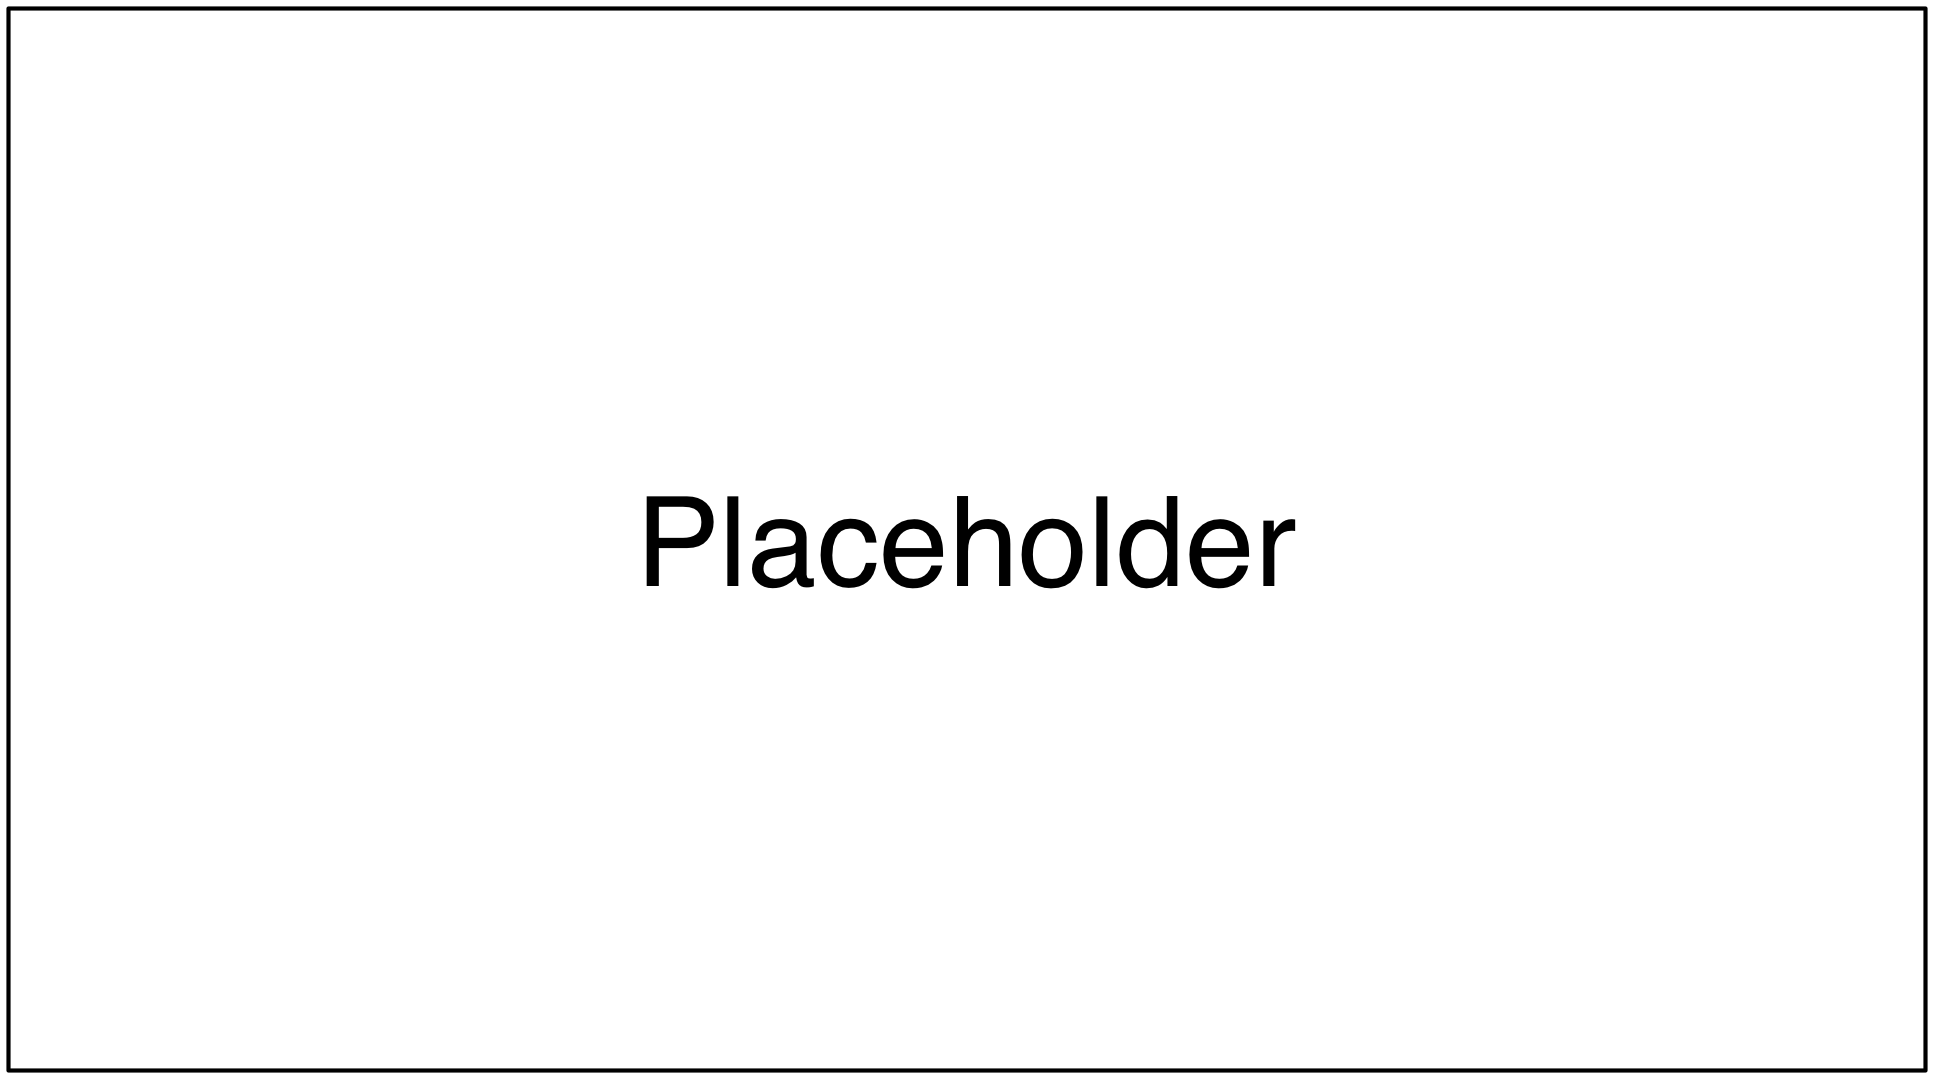
\includegraphics[scale=.5]{figures/placeholder}
	\caption{Our Pure Pursuit Figure}
\end{figure}


Thus, the new vehicle controllers can be specified as follows:
\begin{gather}
\delta(t) = tan^{-1}\left(\frac{2(l_f+l_r)sin(\alpha(t))}{k_{pp}l_d}\right)
\\
a_x(t)=k_6(v_d(t)-v(t))
\end{gather}
%\noindent Given the relations: $x^2+y^2=l^2$ and $x+d=r$, the desired curvature is:
%\begin{align}
%\gamma=\frac{2x}{l^2}
%\end{align}



%Thus, the feedback to the system are the lateral and longitudinal tracking errors. We derive the following results as in  \cite{Snider2009}:
%\begin{gather}
%	\epsilon_x=cos{(\Psi_d)}(s_{x,d}-s_x) +sin{(\Psi_d)}(s_{y,d}-s_y)
%	\\
%	\epsilon_y=-sin{(\Psi_d)}(s_{x,q}-s_x)+cos{(\Psi_d)}(s_{y,d}-s_y)
%\end{gather}

%\noindent Thus, given the vehicle pose and the next waypoint. We must compute $\left\{\Psi_d, \dot{\Psi}_d, s_{x_d}, s_{y_d},\right\}$. 

%This implies that:
%\begin{equation}
%	\theta(0) = sin^{-1} \left(\frac{s_y-c_y}{r}\right)
%\end{equation}
%Then we compute 
%\begin{equation}
%\Psi_d(t) =  \frac{\pi}{2}-\theta(t), t \geq 0
%\end{equation}
%For an arc subtended by the angle $\theta(t)$, the length of the arc, $\rho$ is:
%\begin{equation}
%	\rho = \theta(t) \cdotp r
%\end{equation}
%Alternately one might compute the length of the arc by integrating the velocity as directed along the arc such that $\rho(t) = \int_{0}^{t}v(\alpha) d\alpha$. Now we let $v(\alpha) = v_d$ and hold $v_d$ to be constant. Thus:
%\begin{equation}
%	\rho(t) = v_d \cdotp t
%\end{equation}
%Which implies that:
%\begin{equation}
%	\Psi_d(t) = \frac{\pi}{2} - \left( \theta(0) + \frac{v_d \cdotp t}{r}\right)
%\end{equation}
%Differentiating we conclude that:
%\begin{equation}
%	\dot{\Psi}_d = -\frac{v_d}{r}
%\end{equation}
%\begin{figure}
%	\centering
%	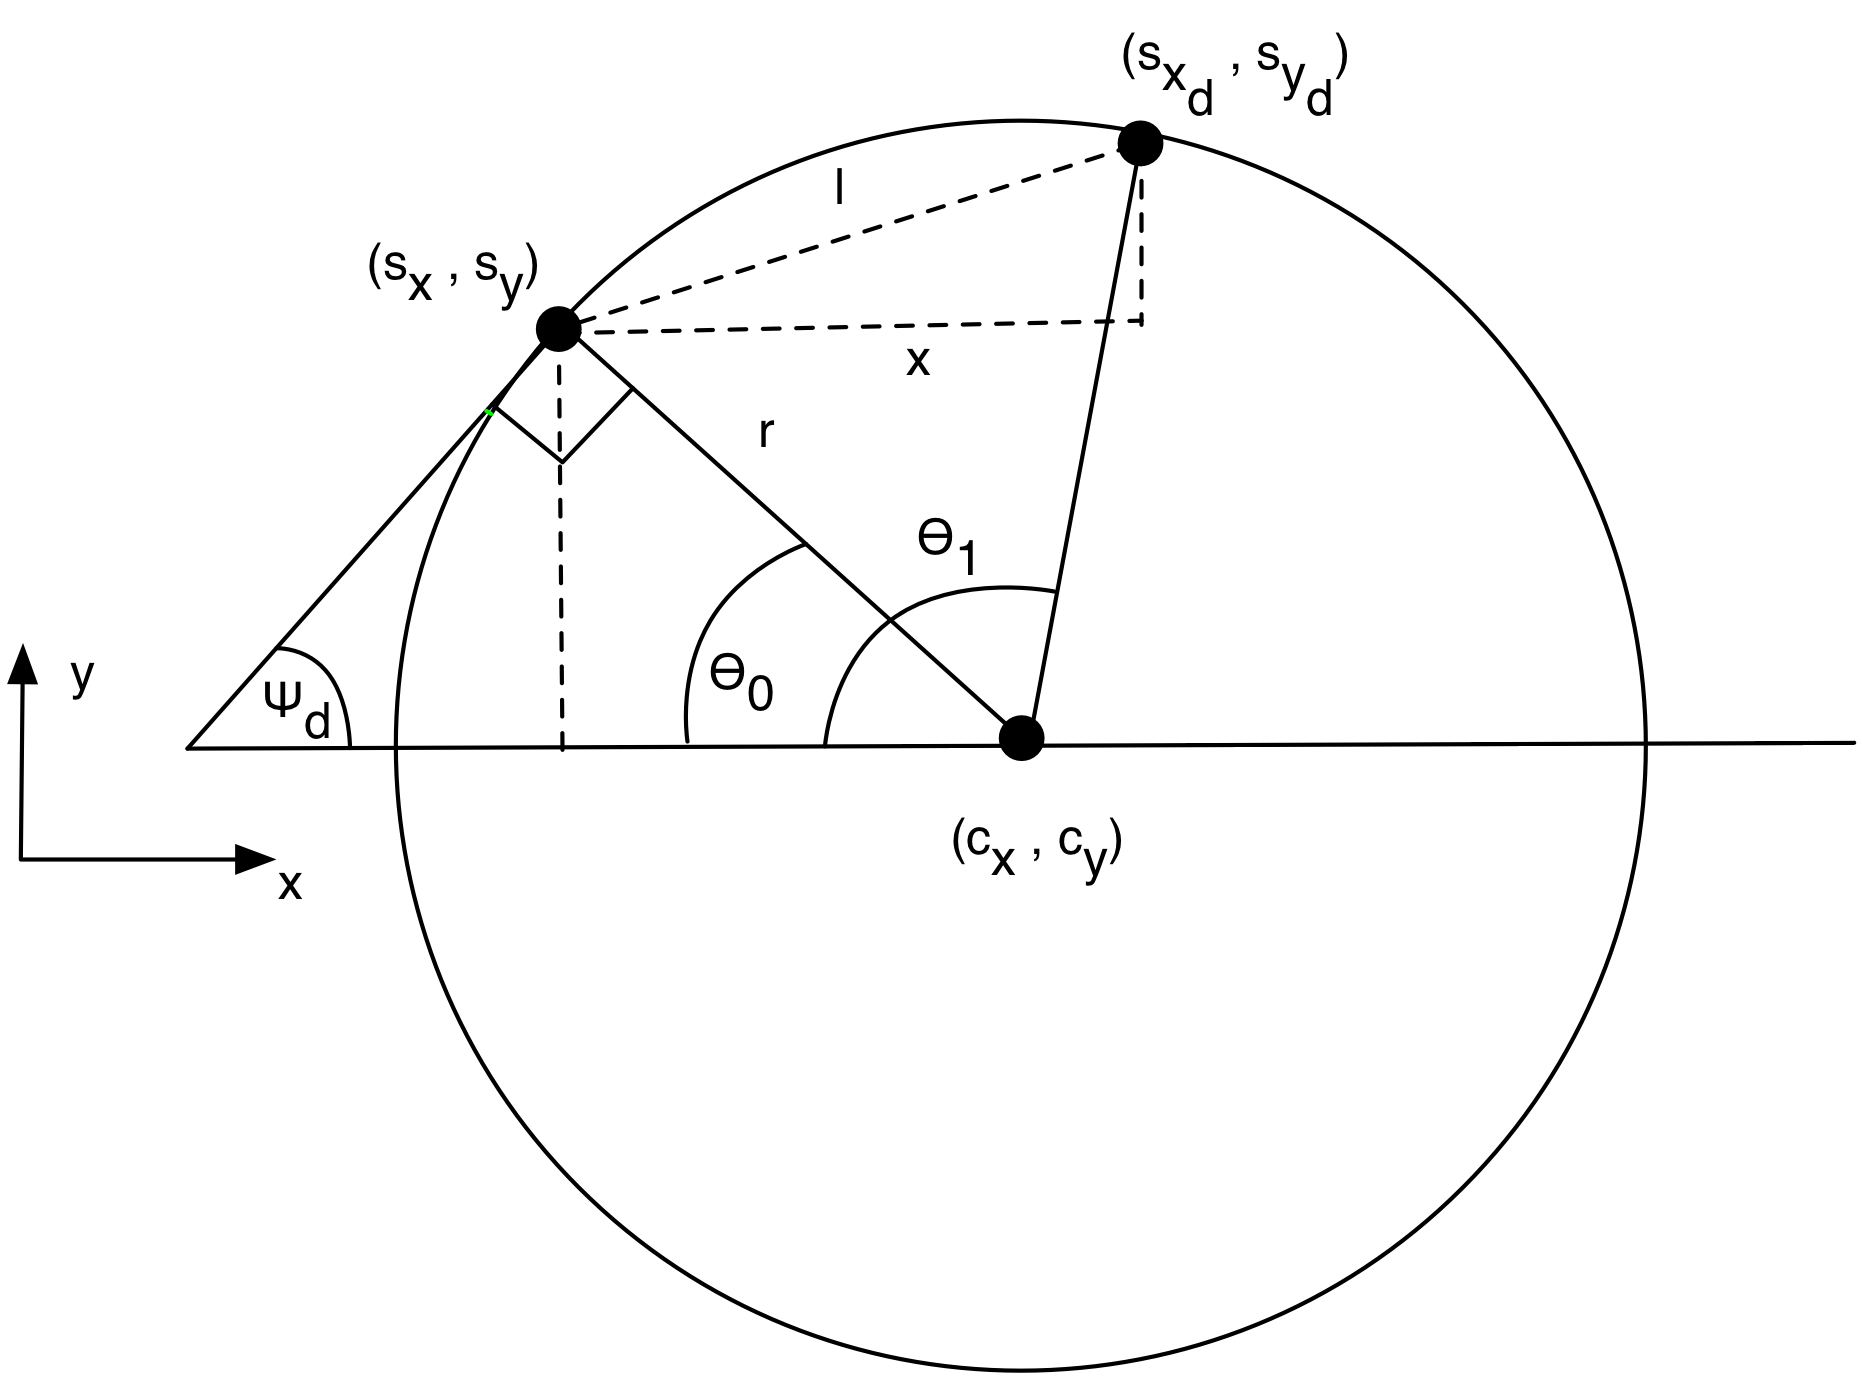
\includegraphics[scale=0.5]{figures/traj-track-diagram}
%	\caption{Geometric Description of Ego-Vehicle Trajectory Geometry}
%\end{figure}

%\noindent Thus we can derive the remaining equations for a point mass moving in a plane:
%\begin{gather}
% \dot{\Psi}_d= -v_d/r\\
% \dot{s}_{y_d} = v_d \left(sin(\Psi_d) \right)\\
% \ddot{\Psi}_d = 0
%\end{gather}